\documentclass[a4paper]{article}

\usepackage[]{graphicx}
\usepackage[style=apa]{biblatex}
\usepackage[colorlinks=true,citecolor=blue,linkcolor=blue]{hyperref}
\usepackage[]{microtype}
\usepackage[table]{xcolor}
\usepackage[]{multicol}
\usepackage[toc,page]{appendix}
\usepackage[capitalise]{cleveref}
\usepackage[]{float}
\usepackage[]{setspace}
\usepackage[]{latexsym}

\graphicspath{{./graphs/}{./images/}}
\addbibresource{final-report.bib}

\begin{document}
\begin{titlepage}
  \centering
  \Large{Raffles Institution \\ Year 2 Research Education \\ Final report} \\
  
\includegraphics[scale=0.5]{ri-school-crest.png} \\
  \huge{How to harness green roof technology in schools to encourage
    Singaporean students, through CCAs, to play an active role in reducing
    carbon footprints and controlling the negative effects of greenhouse
    gases?
  } \\
  \vspace{1cm}
  \large{
    \textbf{Authors}: \\
    Nathaniel Chong(3) \\
    Lee Jun Wei(13)\footnote{Group leader} \\
    Teng Zi Huan(28) \\
    Isaac Yeo(32) \\
    \vspace{1cm}
    \begin{tabular}{r@{:}l}
      \textbf{Class} & \hspace{1cm} 2F \\
      \textbf{Teacher} & \hspace{1cm} Dr. Tan Guoxian \\
    \end{tabular}
  }
\end{titlepage}

\newpage

\begin{abstract}
  \noindent
  In Singapore, many students do not see the need to protect the
  environment. Thus, this study seeks to investigate the feasibility of
  educating Singapore youth about the environment and encouraging them
  to play an active role in environmental protection through the use of
  green roofs in schools. Surveys were conducted, and most respondents
  were secondary school students. An interviews was also conducted
  with two interviewee from secondary school to gain insight into
  the matter. After further analysis, it was observed that most did
  not really know about green roofs, but had a positive perception of
  green roofs. They also had moderate environmental awareness. Thus,
  active participation in environmental protection through the use
  of green roofs should be possible with more education about green
  roofs and the severity of climate change, and how to play an active
  role in minimising their carbon footprint.
\end{abstract}

\newpage

\tableofcontents

\newpage

\begin{multicols}{2}

  \section{Introduction}
  \subsection{On green roofs}
  \subsubsection{Definition}
  \paragraph{} Green roofs involve growing plants on roofs, which can
  be sorted into muscinal roofs, herbaceous roofs and arbustive roofs
  \parencite{ecoeng}.


  \subsection{Benefits}
  \paragraph{} They can reduce energy demand on space conditioning,
  help in purifying air, and if widely adopted, could reduce the urban
  heat island effect, among other benefits \parencite{energeff}. These
  benefits will be further looked into in \cref{sec:grben}.


  \subsection{Purpose and significance of research question}
  \subsubsection{Purpose}
  \paragraph{} To find ways to, through green rooftop technology, increase
  Singapore students' awareness of climate change and how they can play
  a part in reducing it. See below for more information as to how this
  topic is relevant to today's dynamic and modern society.

  \subsubsection{Significance}
  \paragraph{} Understanding climate change is of significant importance
  in today's society, as it poses a large problem to the environment.
  We think that harnessing green roofs may be able to encourage students
  to take action against this. The effects of climate change and how green
  roofs can help are further studied in \cref{sec:grhelp}.

  \subsection{Target Audience} \label{ssec:target-aud}
  \paragraph{} We chose primary and secondary school CCAs as our target audience as
  they are old enough and mature enough to understand the implications
  of global warming and climate change, and global warming. They will
  also be the leaders of tomorrow, so it is even more important for them
  to understand this.


  \subsection{Adoption}
  \paragraph{} If adopted in schools by having students to take care
  of and keep up the green roofs, the students would then build this
  habit of caring for and maintaining a green roof, something they would
  hopefully continue to do upon reaching adulthood in the future when
  they would be able to realise human impact on the environment. This is
  even more important should they become national leaders, who have the
  power to influence the lives of other people. Having this influence
  from young, they would then turn to such technologies which can affect
  climate change for the better.

  \section{Literature review}
  \subsection{Further study of the benefits of green roofs} \label{sec:grben}
  \subsubsection{Economic}
  \paragraph{} Research on green roof technologies has so far proven them
  beneficial, with \cite{energeff} mentioning that they can reduce energy
  demand on space conditioning and decrease temperature fluctuations. This
  is agreed on by \cite{CFGRSG} who states that increased roof insulation
  could reduce space conditioning required in the building. Other
  sources also mention the decreased carbon emissions due to lower energy
  consumption from improved thermal performance \parencite{CommAwareGBSyd}
  which reduces cost of energy as there will be up to a 75 percent
  decrease in energy usage for cooling the building, with daily averages
  dropping from 7.5kWh to 1.5kWh \parencite{energeff}. \cite{energeff} also
  mentions that daily temperature fluctuations on roofing membranes are
  significantly reduced, which can increase the lifespan of the roof.


  \subsubsection{Environmental}
  \paragraph{} \cite{energeff} states that if green roof technologies
  are widely adopted, they could reduce the urban heat island effect (a
  situation where an urban area has higher temperatures than surrounding
  rural areas) by having the plants on the green roofs absorb some of the
  heat. \cite{HKGreenRoofGL} also suggests that it ``mitigates the urban
  heat island effect''. It is also said that green roofs can increase the
  aesthetics of urban landscape, reduce glare for surrounding buildings,
  showing its importance and relevance in today's highly urbanised
  society. Additionally, \cite{HKGreenRoofGL} found that green roofs
  can mitigate air quality issues, which are important for the wellbeing
  of all. Therefore, we find that there is a need to educate students,
  especially those in secondary institutions (as they are mature enough to
  understand the gravity of global warming and climate change and the need
  to take immediate action, and are more likely to have time to undertake
  this project than those in tertiary institutions) about green roofs.
  Vegetation on green roofs help purify the air and convert carbon
  dioxide into oxygen, which reduces the amount of greenhous gases in
  the air. \parencite{energeff} mentions this, and \cite{CommAwareGBSyd}
  goes a step further, even suggesting that green roofs help achieve zero
  carbon footprints. The plants also take in rainwater, reducing the
  water in the sewage system which needs to be purified and discharged
  to the sea, helping to stabilize the groundwater level and reducing
  the possibility of the sewer clogging and malfunctioning.


  \subsection{Climate change and how green roofs can prevent it} \label{sec:grhelp}
  \paragraph{} According to \cite{nasa}, at the rate of climate
  change we are at, the sea levels worldwide would increase by 1--4
  feet. This leads to the question of whether Singapore would truly
  be safe in the future. This thus draws the necessary attention and
  action of the Singapore Government and the citizens. Actions required
  includes educating the youth of the society of the consequences of
  climate change and the possible course of action.  However, students
  in Singapore have ``major gaps in their understanding [of climate
  change]''\parencite{student_carbon_footprint}, and thus will not
  see the need to protect the environment and prevent it. Therefore,
  it is necessary for us to research methods that can be used to raise
  awareness of climate change in Singaporean students. At the same
  time, we believe that green roofs can be an effective measure in
  fulfilling its purpose in combating climate change and in motivating
  the Singaporean youth to play an active role in it. Green roofs are a
  potential way to not only encourage the next generation of Singaporeans
  to take climate action,  when the country is in their hands. Proper
  education of the youth would, hopefully, eventually lead to a rise in
  green technology and build a greener, healthier world for everyone
  to live in, one that is possibly freed of the grasps and struggles
  of climate change. Even in Singapore, green roofs have been utilised
  on buildings such as the Nanyang Technological University's School
  of Art, Design and Media. According to \cite{greenbuild_advant1},
  green roofs not only play a part in helping to slow climate change,
  they also help create a better environment for residents.




  \section{Methodology}
  \subsection{Purpose}
  \paragraph{} We believe that green roofs are severely underused
  in Singapore despite the advantages, and think that schools are a
  great place to have them implemented. The surveys and interview we
  conducted were in order to find out Singaporean students' awareness
  and perception of green roofs, as well as the viability of, and their
  willingness to assist in green roof projects in schools.

  \subsection{Interview}
  \paragraph{} An interview was conducted, on 28 June at 3pm. As
  the interviewee was unable to use Microsoft Teams due to a lack
  of access, we used other means to conduct the interview, such as
  Zoom or Discord video calls. The interviewee was a boy studying in
  West Spring secondary. During the interview, the interviewee was
  asked questions regarding the features, advantages, disadvantages and
  possible hindrances in their implementation. He was also asked about
  how he felt about implementing them on school roofs, and how he thought
  other students might feel about it.

  \subsection{Surveys}
  \paragraph{} The survey respondents came from two different age
  groups: primary and secondary school students. In total, we received
  survey responses from 21 students, one of which was not a serious
  response (evident from the options selected, which were all falling
  in the ``1'', ``False'', or similar categories,
  even disagreeing to the PDPA clause). Hence, we chose to omit
  the data gathered from that respondent and focus on the other 20
  respondents. However, 19 of the remaining 20 respondents indicated that
  they were of 13--17 years of age, and hence the demographics of our
  survey were quite limited and the data collected may (unfortunately) not
  be representative of the entire student population in Singapore. The
  questions to gauge their understanding were based on two research
  papers by \cite{HKGreenRoofGL} and \cite{energeff}.



  \section{Results and analysis}
  \subsection{Summary and results}
  \subsubsection{Surveys}

  \begin{figure}[H]
    \centering
    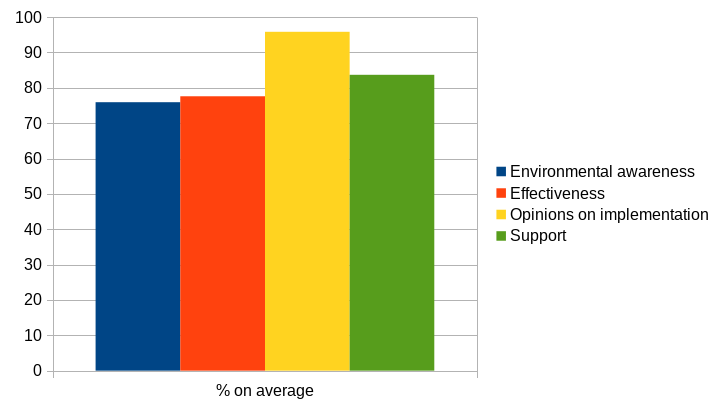
\includegraphics[width=\linewidth]{responses-ave.png}
    \caption{What respondents think of green roofs on average}
    \label{fig:surv-resp}
  \end{figure}

  \begin{figure}[H]
    \centering
    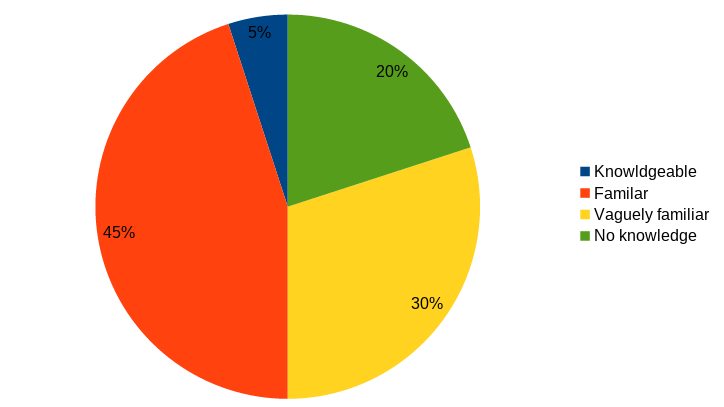
\includegraphics[width=\linewidth]{knowledge.png}
    \caption{Knowledge levels of respondents}
    \label{fig:know-levels}
  \end{figure}

  \begin{figure}[H]
    \centering
    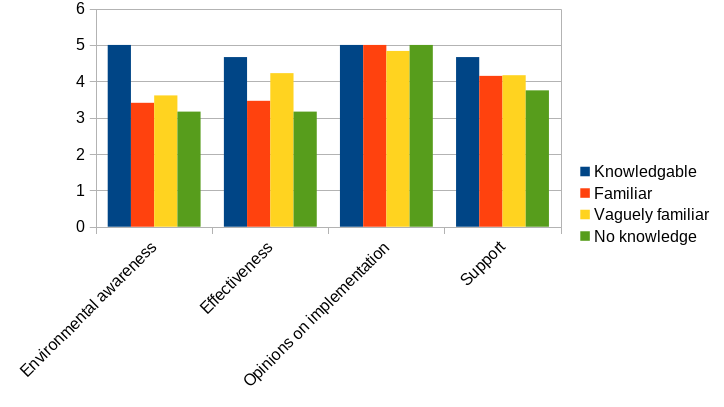
\includegraphics[width=\linewidth]{knowledge-opinions.png}
    \caption{
      Subgroup analysis of \cref{fig:surv-resp}: knowledge of respondents
      against what they think of green roofs
    }
    \label{fig:know-opn}
  \end{figure}

  \begin{figure}[H]
    \centering
    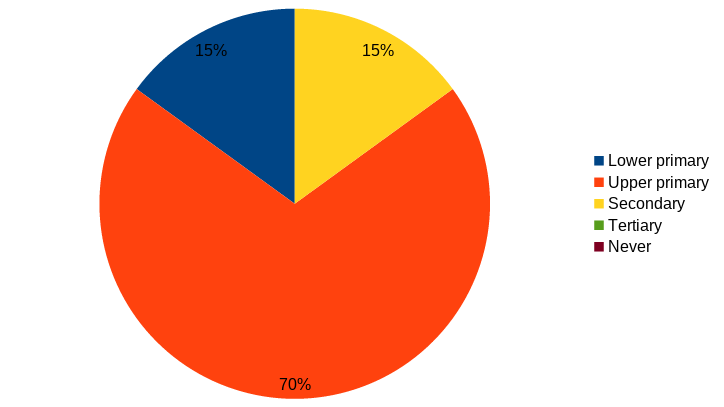
\includegraphics[width=\linewidth]{level.png}
    \caption{
      Respondents' opinions on when students should start getting involved
      in maintaining green roofs
    }
    \label{fig:levels}
  \end{figure}

  \subsubsection{Understanding and support of green roofs}
  \paragraph{} The results also show that not many students
  have a good understanding of how green roofs work (as shown in
  \cref{fig:know-levels}), but are able to identify its benefits towards
  climate change, and would actively participate in reducing carbon
  footprint if green roofs were to be implemented in schools. This shows
  that people do not need to have a good understanding of green roofs,
  but only a general understanding that it benefits the environment and
  by helping maintain the conditions of green roofs would reduce carbon
  footprint. Unsurprisingly, the single respondent who indicated that
  he was ``knowledgable'' about green roofs was the most optimistic,
  fully agreeing to most of the statements. Furthermore, as is shown in
  \cref{fig:know-opn}, respondents with more knowledge of green roofs
  were, on average, more environmentally aware and showed more support,
  and thought they were more effective in general.

  \subsubsection{
    When students should start their involvement in maintaining green
    roofs
  }

  \begin{table*}
    \centering
    \caption{Number of respondents willing to do each maintenance duty}
    \begin{tabular}{|c|c|c|c|c|}
      \hline
      \rowcolor{cyan}
      Pest control & Pruning vegetation  & Adding compost &
      Monitoring plant growth & None of the above \\ \hline
      12 & 12 & 11 & 12 & 2 \\ \hline
    \end{tabular}
    \label{tab:duties}
  \end{table*}

  \paragraph{} \label{par:support} In general, we found that the
  majority of Singaporean students are supportive of the concept of
  green roofs, from \cref{fig:surv-resp}.

  \subsubsection{Interview}
  \paragraph{} The interviewee, who was quite knowledgeable
  regarding green roofs, responded by saying that green roofs served
  several purposes: collecting water and acting as insulators, among
  others. However, they also cost a lot to build, and require a lot of
  maintenance. Despite those disadvantages, he thought that they should
  be implemented on school roofs as they could reduce the amount of
  electricity spent on electricity as they act as an insulator, thus
  reducing costs.



  \subsection{Analysis}
  \paragraph{} These results showed that in general, teenagers in
  Singapore were supportive of implementing green roofs. When asked
  about the practical usage of green roofs, 95\% of respondents agreed
  on all aspects meaning that they believed green roof systems being
  implemented would be a good idea. The one respondent that did not agree
  on every aspect noted that building green roofs was a waste of effort,
  but agreed on all other parts. As is evident from \cref{tab:duties},
  most respondents were rather willing to participate in the maintenance
  of green roofs, with only two respondents indicating their unwillingness
  to participate in the maintenance of green roofs.

  \paragraph{} In \cref{ssec:target-aud}, we mentioned that our target
  audience would be primary or secondary school CCAs, as they would be
  more mature in thought and not as stressed as their seniors. However,
  as is shown in \cref{fig:levels}, survey results seem to suggest that
  students be introduced to maintaining green roofs at the upper primary
  level instead. After some thought, we decided that this would indeed
  be more appropriate, as environmental awareness should be instilled
  in youth from a young age.

  \paragraph{} The interviewee mentioned that green roofs would provide
  a better environment for students to learn in. This is presumably
  because green roofs act as insulators and can thus help keep air in the
  classroom cool naturally. He also mentioned that he did not know any
  schools that implemented green roofs. This shows that green roofs have
  not yet been adopted in Singapore schools. This is supported by ``I
  highly doubt that it would actually be implemented as my school likes
  spend more of their budget on certain CCAs, but not on green roofs'',
  implying that schools in Singapore do not yet realise the benefit of
  having green roofs.



  \section{Discussion and implications of findings}
  \subsection{General perception of green roofs}
  \paragraph{} \cite{CommAwareGBSyd} found that 55 percent of
  respondents to a survey conducted ``strongly agreed'' that greenery
  was important and its benefits outweighed its additional costs,
  showing public support of this idea suggesting that our idea may be
  quite welcome. This is supported by \cite{CFGRSG}, who said that with
  therapeutic value of greenery in reducing stress already established,
  green roofs are used commonly in Singapore to soften the harsh
  urban environment and to improve the quality of life. Modern green
  roofs are now mainly based on cost, energy, water savings and carbon
  reduction \parencite{CFGRSG}.  71.8 percent of respondents in a survey
  conducted by \cite{CommAwareGBSyd} stated that greenery would make
  a place more attractive to live in meaning that greenery could have
  a positive impact on people's lives, especially for students who
  spend time in school. However, \cite{GRBuildEnSave} also found that
  33.8 percent of respondents to their survey had less than a general
  understanding of the concept of green roofs--- with the oldest(76+)
  and youngest(12--17) age groups showing the least understanding,
  further stressing the need to educate students about green roofs,
  although this may be inaccurate due to the small sample size. However,
  \cite{student_carbon_footprint}, also found that students in Singapore
  do not fully understand climate change.



  \subsection{Possible implementations}
  \paragraph{} We propose that students be grouped according to three
  different CCA groups: sports, performing arts and uniformed groups,
  with each group doing its own part. The students in sports CCAs
  and uniformed groups will carry out the physically more demanding
  tasks (e.g.doing the actual planting itself and taking part in
  maintenance with the assistance of professionals, etc.) since they
  are more used to carrying out such physical tasks than the students in
  performing arts CCAs. The students in performing arts CCAs can manage
  the logistics(planning projects, budgets, etc.) seeing that they are
  likely to be less physically inclined while everyone still keeping to
  the recommended guidelines by \cite{HKGreenRoofGL}.



  \paragraph{} We also think that more education to students about
  green roofs is necessary in order for them to fully understand their
  benefits. As shown in \cref{par:support}, students were generally more
  supportive of green roofs if that had more knowledge of them. However,
  \cref{fig:know-levels} clearly shows that most students are lacking in
  knowledge of green roofs. Therefore we view further education on
  green roofs essential to achieving greater support for green roofs
  amongst students, thus making it more likely for them to be willing
  to participate actively.

  \section{Limitations}
  \paragraph{} As we only had a limited amount of time, we may have collected
  insufficient data to fully justify our conclusion, hence the conclusion may
  not be entirely reliable; we only had 21 responses to the survey, one of
  which was illegitimate.
  \section{Conclusion}
  \paragraph{} Current research has shown that green roofs can be
  beneficial by maintaining a stable temperature, reducing space
  conditioning, amongst other benefits. However, there is still
  a knowledge gap where Singaporean students' perceptions of green
  roofs and its viability in schools are not addressed which is why our
  research is relevant and necessary.

  \paragraph{} Our research suggests that students should be further
  educated on the severity of climate change, the pressing need to protect
  the environment, and of course, the benefit of green roofs. Upper
  primary students and perhaps secondary students should also play an
  active role in maintaining green roofs, which should be implemented
  in schools, so as to instil a sense of responsibility for protecting
  the environment, and have them develop a habit of caring for it and
  playing an active role in preventing climate change.


\end{multicols}

\newpage

\printbibliography[heading=bibintoc,title={References}]

\newpage

\begin{appendices}
  \section{Survey questions}
  We are a group of Year 2 Students from Raffles Institution, and we
  would like to conduct this survey in order to gain important insights
  into the public perception of green roof technologies. Our project is
  centred around how the Singaporean public views green roofing and the
  viability of their implementation in schools. In this survey, we are
  talking about green roofs of the intensive type, where a variety of
  plants will be grown on a rooftop, instead of just grass.

  All information collected will be kept strictly confidential and
  anonymous, with consent given, and will be for the sole purpose of
  conducting our research. The information will not be shared to any
  third party and we will not retain the information for longer than we
  need it in order to finish our research. Participation in our survey is
  consensual and voluntary, and I agree that the information shared here
  can be collected, used and disclosed to the relevant parties for the
  aforementioned research. Your consent for the above may be withdrawn at
  any point during the survey.

  We would greatly appreciate it if you took a few minutes to complete
  this survey. Thank you for your time and effort.

  \begin{itemize}
    \item[Q1.] What is your age? \\ $\Box$ 12 years old and below \\
      $\Box$ 13-16 years old \\ $\Box$ 17-18 years old \\ $\Box$ 19-21
      years old \\ $\Box$ Above 21 years old

    \item[Q2.] What category of Co-Curricular Activity(CCA) do you take
      part in? (Tick all that apply) \\ $\Box$ Sports \\ $\Box$ Performing
      arts \\ $\Box$ Uniformed groups \\ $\Box$ Clubs, societies and
      associations \\ $\Box$ Others \\ $\Box$ No CCA/Not applicable

    \item[Q3.] On a scale of 1 (strongly disagree) to 5 (strongly agree),
      please indicate how strongly you agree with the following statements:
      \begin{table}[H]
        \begin{tabular}{|p{0.6\linewidth}|c|c|c|c|c|}
          \hline
          Statement & 1 & 2 & 3 & 4 &
          5 \\ \hline

          The environment is in an undesirable and adverse situation. &
          $\Box$ & $\Box$ & $\Box$ & $\Box$ & $\Box$ \\ \hline

          There are technologies available that can improve the state of
          the environment. & $\Box$ & $\Box$ & $\Box$ & $\Box$ & $\Box$
          \\ \hline

          Our environment can be improved through the use of green roofs. &
          $\Box$ & $\Box$ & $\Box$ & $\Box$ & $\Box$ \\ \hline
        \end{tabular}
      \end{table}

    \item[Q4.] How familiar are you with the concept of green roof
      technologies? \\ $\Box$ Never heard of them before this survey. \\
      $\Box$ I vaguely know what they are. \\ $\Box$ I know some details on
      what they are and how they function. \\ $\Box$ I can describe in some
      detail what green roofs are,  their uses, and their advantages and
      disadvantages. \\ $\Box$ I have experience and knowledge in the field
      of green roofing, whether as part of my occupation or as research done.

    \item[Q5.] On a scale of 1 (strongly disagree) to 5 (strongly agree),
      please indicate how strongly you agree with the following statements:
      \begin{table}[H]
        \begin{tabular}{|p{0.6\linewidth}|c|c|c|c|c|}
          \hline
          Statement & 1 & 2 & 3 & 4 &
          5 \\ \hline

          Green roof technology can reduce the effect of greenhouse
          gases on the environment. &
          $\Box$ & $\Box$ & $\Box$ & $\Box$ & $\Box$ \\ \hline

          Green roof technology can reduce the cost of running a building.
                 & $\Box$ & $\Box$ & $\Box$ & $\Box$ & $\Box$ \\ \hline

                 Green roof technology, if widely implemented, could help lower
          temperatures in an area of effect.  & $\Box$ & $\Box$ & $\Box$
                                              & $\Box$ & $\Box$ \\ \hline

          Green roof technology can help improve air quality. &
          $\Box$ & $\Box$ & $\Box$ & $\Box$ & $\Box$ \\ \hline

          Green roofs are aesthetically pleasing and can improve the
          visual appearance of a cityscape.  & $\Box$ & $\Box$ & $\Box$
                                             & $\Box$ & $\Box$ \\ \hline
        \end{tabular}
      \end{table}

    \item[Q6.] Please tick under the correct column to specify your
      opinion on the practical use of green roof systems.
      \begin{table}[H]
        \begin{tabular}{|p{0.6\linewidth}|c|c|c|}
          \hline
          Question & True & False \\ \hline
          Do you think green roofs can help improve the environment in
          Singapore? & $\Box$ & $\Box$ \\ \hline

          Do you think it is a waste of materials to try and build green
          roofs on buildings? & $\Box$ & $\Box$ \\ \hline

          Do you think it is a waste of effort to try and build green
          roofs on buildings? & $\Box$ & $\Box$ \\ \hline

          Would you support the government’s hypothetical decision to
          build green roofs on all buildings? & $\Box$ & $\Box$ \\ \hline
        \end{tabular}
      \end{table}

    \item[Q7.] On a scale of 1 (strongly disagree) to 5 (strongly agree),
      please indicate how strongly you agree with the following statements:
      \begin{table}[H]
        \begin{tabular}{|p{0.6\linewidth}|c|c|c|c|c|}
          \hline
          Statement & 1 & 2 & 3 & 4 &
          5 \\ \hline

          More green roofs should be implemented in Singapore. &
          $\Box$ & $\Box$ & $\Box$ & $\Box$ & $\Box$ \\ \hline

          Green roofs should become standard in Singaporean buildings. &
          $\Box$ & $\Box$ & $\Box$ & $\Box$ & $\Box$ \\ \hline
        \end{tabular}
      \end{table}

    \item[Q8.] Please indicate whether you believe that the following
      statement is correct: I believe that my peers will be able to
      effectively care for and maintain a green roof system in a sensible
      manner. \\ $\Box$ True \\ $\Box$ False

    \item[Q9.] When in a student’s schooling life do you think
      green roofs start to be used in schools with student involvement
      in maintaining it? \\ $\Box$ At the lower primary level (Age 7 and
      above) \\ $\Box$ At the upper primary level (Age 10 and above) \\
      $\Box$ At the secondary level (Age 13 and above) \\ $\Box$ At the
      tertiary level (Age 17 and above) \\ $\Box$ Green roof systems in
      schools should NOT involve students. \\ $\Box$ Green roof systems
      should NOT be implemented in schools.

    \item[Q10.] Which of the following tasks would you be willing to
      perform? (Tick all which apply) \\ $\Box$ Pest control(inc. Weeding
      plants, adding pesticide to soil etc.) \\ $\Box$ Pruning vegetation
      \\ $\Box$ Adding compost \\ $\Box$ Monitoring and keeping track of
      the types of plants to ensure the absence of unwanted growths \\
      $\Box$ None of the above

    \item[Q11.] \textbf{PDPA clause:} The responses given in this survey
      are, to the best of my understanding, wholly accurate and truthful,
      and I consent to allow the information shared in this survey to
      be used by the researchers for their research. My participation
      is voluntary. We sincerely thank you for your time taken to
      complete this survey. This data is to be collected for the sole
      purpose of furthering our project on the topic of green roofs,
      and the possibility of their utilisation in schools. Strict
      confidentiality and anonymity of the information shared is
      assured. The personal data will not be shared to any third party
      or transferred overseas, and will not be retained for longer than
      is necessary to pursue our research. Your consent to participate
      in this survey may be withdrawn at any time. If you desire so,
      we could send our final report to you. For any further queries,
      please contact any of us at 24YCHON155F@student.ri.edu.sg,
      24YLEEJ623C@student.ri.edu.sg, 24YTENG305C@student.ri.edu.sg,
      or 24YYEOJ426G@student.ri.edu.sg. Thank you. \\ $\Box$ I agree \\
      $\Box$ I disagree
  \end{itemize}

  \section{Interview transcript}
  \begin{table}[H]
    \begin{tabular}{l @{:    } p{0.8\linewidth}}
      \hline
      \textbf{Interviewer} & What do you think are some advantages of
      green roofs? \\

      \textbf{Interviewee} & They serve several purposes-- collecting
      rainwater, acting as insulators\ldots They help reduce the risk
      of endangered species going extinct and provide better living
      conditions. \\

      \textbf{Interviewer} & Ah, I see\ldots then what are some
      disadvantages then? \\

      \textbf{Interviewee} & They cost a lot to build them and require a
      lot of maintenance. \\

      \textbf{Interviewer} & In that case\ldots How do you think these
      problems could be solved? \\

      \textbf{Interviewee} & Uhh\ldots I'm not really sure\ldots \\

      \textbf{Interviewer} & It's all right. So, do you think it is a good
      idea to implement green roofs on school buildings? \\

      \textbf{Interviewee} & Yes, I do, I think it is a good idea to
      implement green roofs on school buildings as it provides a better
      environment for teachers to teach in, and a better environment
      for students to learn in. They also act as insulators, so they are
      also more eco-friendly than normal roofs, reducing the cost of of
      electricity spent on air conditioners and cooling systems. \\

      \textbf{Interviewer} & Do you know any schools which implement
      green roofs? \\

      \textbf{Interviewee} & No, I don't think so. \\

      \textbf{Interviewer} & Alright then. Would you support their
      implementation in schools then? \\

      \textbf{Interviewee} & I would advocate it, but I highly doubt
      that it would actually be implemented as my school spends more of
      their budget on certain CCAs, but not on green roofs. Otherwise
      it is a very good idea. \\

      \textbf{Interviewer} & Would you be willing to maintain a green
      roof should one be implemented in your school? \\

      \textbf{Interviewee} & Yes, I would, as it benefits everyone and
      I have some spare time. \\

      \textbf{Interviewer} & What about other students? \\

      \textbf{Interviewee} & They may be willing. \\

      \textbf{Interviewer} & If not, how do you think they could be
      convinced or persuaded to help out? \\

      \textbf{Interviewee} & Perhaps a social media campaign could be
      launched to alert them about then benefits of green roofs and ask
      them to help. \\

      \textbf{Interviewer} & And what incentives do you think could help
      attract them? \\

      \textbf{Interviewee} & Perhaps giving out free green tea to do
      maintenance work as students like green tea. \\

      \textbf{Interviewer} & Alright, thank you for your time! Do you
      have anything else to add? \\

      \textbf{Interviewee} & Nope. \\

      \textbf{Interviewer} & Alright, thanks! \\

    \end{tabular}
  \end{table}

  \section{Research project timeline}
  \begin{table}[h!]
    \centering
    \caption{Our Timeline}
    \begin{tabular}{|c|c|}
      \hline
      \rowcolor{cyan}
      \textbf{Time} & \textbf{Goal} \\ \hline
      T1W5--T1W9 & Group Project Proposal \\ \hline
      \rowcolor{gray}
      T1W9--T2W3 & Literature review \\ \hline
      T2W3--T2W7 & Finish finalised survey \\ \hline
      \rowcolor{gray}
      T2W7--T3W1 & Administer survey \\ \hline
      T3W1--T3W4 & Data analysis \\ \hline
      \rowcolor{gray}
      T3W3--T3W9 & Prepare for oral assessment \\ \hline
      T3W4--T3W10 & Finalise written report \\ \hline
    \end{tabular}
    \label{tab:timeline}
  \end{table}
\end{appendices}


\end{document}
